\section{Results}

The mostly cytoplasmic deacetylase HDAC6 plays an important role in the management of misfolded proteins and the stress response: it is a critical component of the aggresome pathway \cite{kawaguchi2003deacetylase} and it participates in the formation of stress granules \cite{kwon2007deacetylase, saito2019acetylation}. HDAC6 exerts its diverse biological functions by deacetylating various substrates such as tubulin, HSP90 or cortactin \cite{hubbert2002hdac6, kovacs2005hdac6, zhang2007hdac6, zhang2003hdac}, and also by binding to unanchored ubiquitin chains via a conserved zinc finger domain \cite{hook2002histone, seigneurin2001identification}. During influenza A uncoating after membrane fusion in late endosomes, HDAC6 mediates physical connections between the virus and molecular motors such as dyneins and myosins (Figure \ref{figure:fluUncoating}). To approach a mechanistic and quantitative understanding of HDAC6-mediated uncoating, we first asked whether it is physically plausible that molecular motors exert sufficient forces on the viral M1 capsid for its breakage. In a tug-of-war scenario, forces exerted by these motors could break the M1 capsid and release the viral ribonucleoprotein (RNP) complex (Figure \ref{figure:fluUncoating}) \cite{banerjee2013high}.

\begin{figure}
\begin{center}
\includegraphics[width=0.8\textwidth, trim={1.0cm 1.0cm 1.0cm 1.0cm}, clip]{D_chapters/1_TugOfWar/SchematicUncoating.pdf}
\caption[HDAC6-mediated influenza A virus M1 capsid disassembly mechanism]%
{Schematic representation of HDAC6-mediated influenza A virus M1 capsid disassembly mechanism, adapted from \cite{banerjee2014influenza}. \par Influenza virions enter the host cell through receptor-mediated endocytosis. An endosome with the viral particle is transported along microtubules by the molecular motors dynein and kinesin. Endosomal acidification during the transport towards the cell nucleus primes the viral core for uncoating via the influx of protons and potassium into the core through the viral M2 channel. At the critical pH, viral HA triggers fusion of the viral envelope with the endosomal membrane, forming a fusion pore and exposing the viral matrix protein M1 to the cytosol. The virus mimics misfolded proteins by carrying unanchored ubiquitin (Ub) chains. The current conceptual model assumes that HDAC6 binds these Ub chains and recruits molecular motors dynein and myosin 10 for the transport along microtubules towards the aggresome \cite{banerjee2014influenza} - a perinuclear assembly of misfolded proteins at the microtubule organizing center (MTOC). Forces exerted by the motors break the viral capsid and thereby release viral genetic material. Adapted from \cite{banerjee2014influenza}}
\label{figure:fluUncoating}
\end{center}
\end{figure}

To represent the underlying biophysics of a tug-of-war mechanism, we developed a mathematical model. It features the capsid at the stage when it is exposed via the fusion pore, interactions between the capsid and molecular motors, and interactions between motors and the host cell’s cytoskeleton (Figure \ref{figure:fluMassSpring}A). Specifically, we assume that M1 proteins (the masses) are arranged in a regular mesh approximately of the size of the fusion pore \cite{hilsch2014influenza}; they are connected to each other by elastic bonds (springs with Morse potentials; see Methods \ref{ch:TugOfWarMethods} for details). We represent the cytoskeleton by a single, randomly directed microtubule and by a denser network of actin filaments with a randomly located nucleation point. Molecular motors can be connected (directly or indirectly, which we do not distinguish in this model) to the M1 proteins exposed to the cytoplasm and to the cytoskeleton, and thereby exert forces. Specifically, dynein motors can walk along the microtubule in a single direction, while myosin motors can walk along actin filaments in random directions. We compute the resulting forces through a tug-of-war model with experimentally determined motor characteristics \cite{gennerich2007force, muller2008tug, norstrom2010unconventional}, which we modified to represent dyneins, kinesins, and positive- and negative-direction myosins. Importantly, the model considers that the force exerted by each individual motor depends on all the other motors bound to the same cargo. If these combined motor forces lead to the distance between any two neighboring M1 nodes exceeding the diameter of the viral ribonucleoprotein (RNP) complex for a sufficient duration, we classify the capsid as broken (see Methods \ref{ch:TugOfWarMethods} for details).

\begin{figure}
\begin{center}
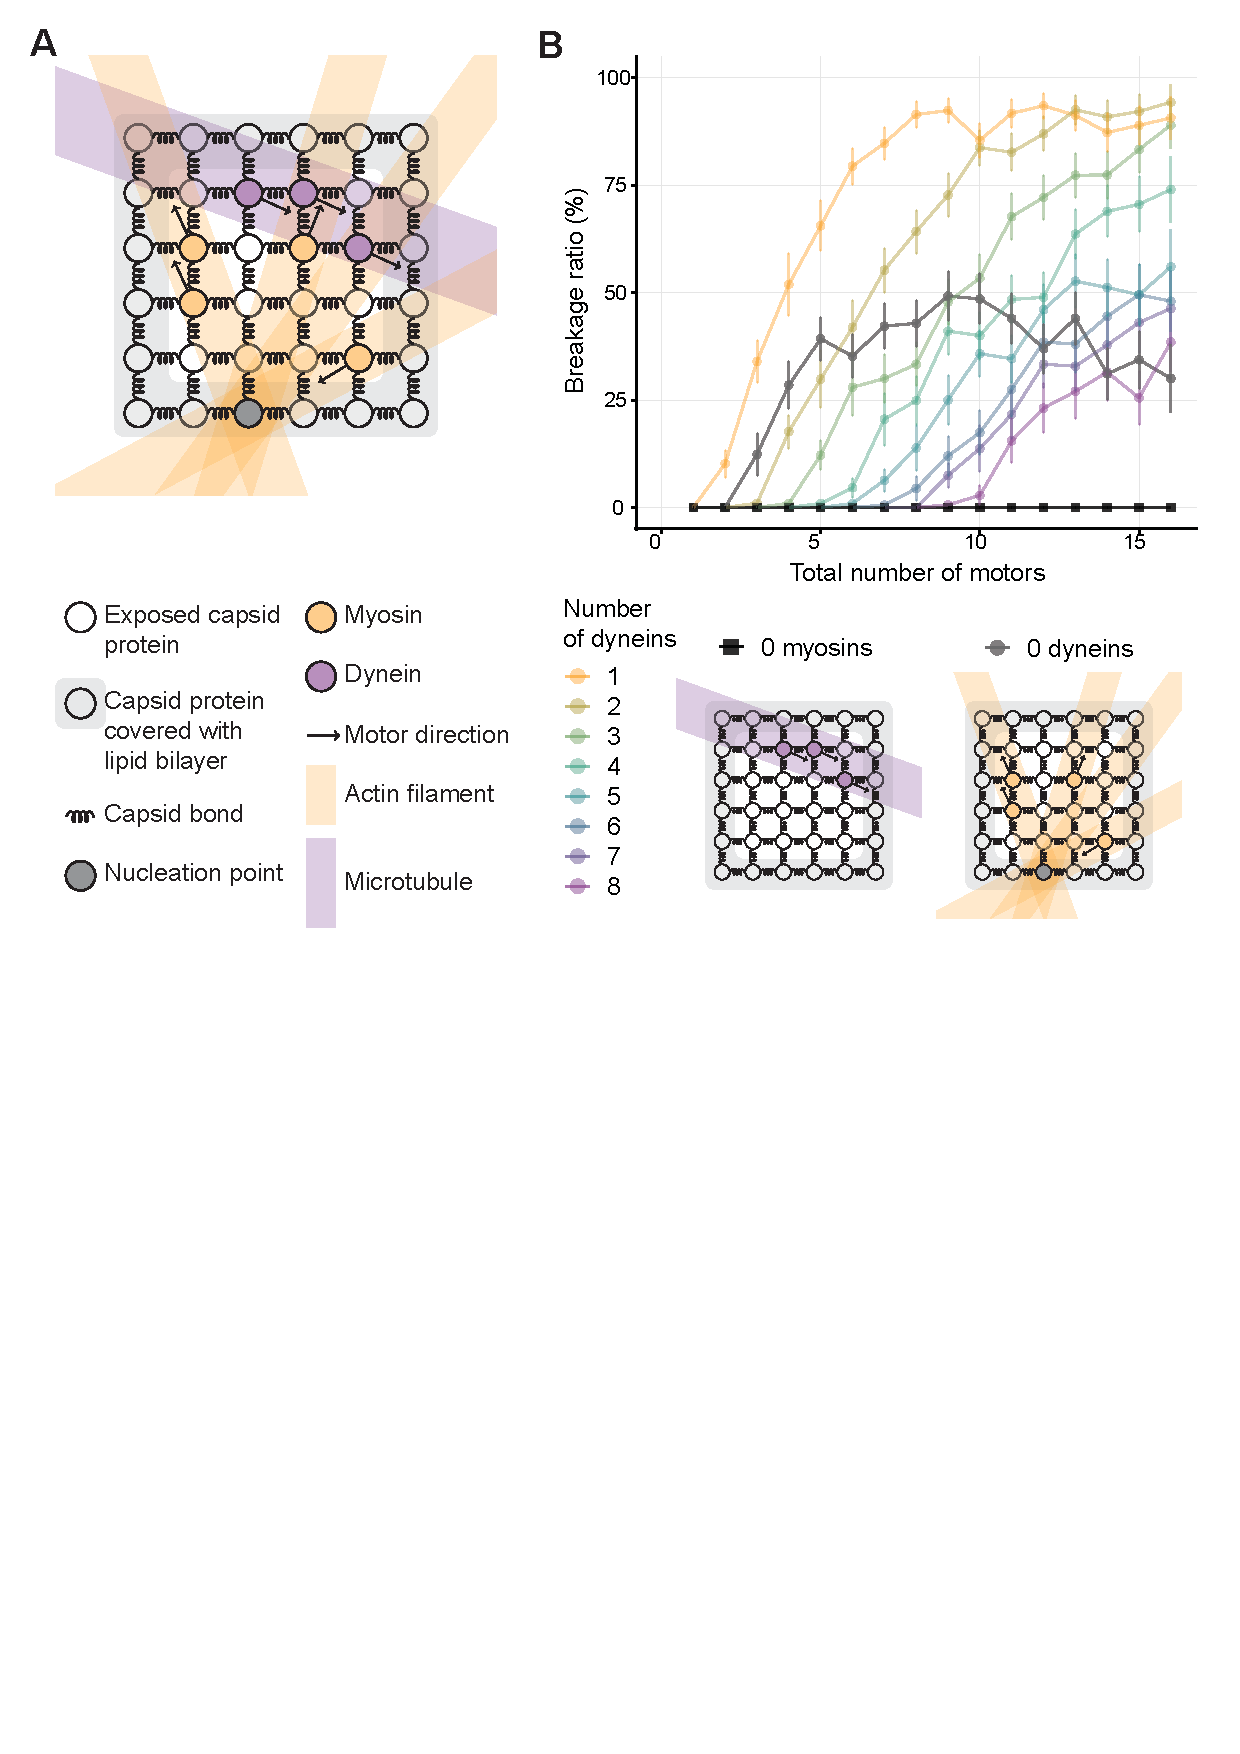
\includegraphics[width=0.95\textwidth, trim={0cm 13.5cm 0cm 0cm}, clip]{D_chapters/1_TugOfWar/FIGURE2_upd.pdf}
\caption[A mass-spring model for capsid-motor interactions predicts that motor forces suffice for efficient virus uncoating]%
{A mass-spring model for capsid-motor interactions predicts that motor forces suffice for efficient virus uncoating. \par
(A) Structure of the two-dimensional viral capsid model. Exposed M1 protein in the viral capsid is represented as a square grid with edges anchored in the lipid bilayer. One microtubule is randomly oriented relative to the capsid. Dynein and myosin motors are attached to the exposed capsid proteins. Dyneins are only able to move along the microtubule, while myosins can move in any direction along the dense actin filament network anchored at the fusion pore with the nucleation point (see Methods \ref{ch:TugOfWarMethods} for details).\par
(B) Predicted capsid breakage probabilities for varying numbers of myosin and dynein motors, and combinations thereof, when they are attached to the capsid. Simulation results are presented as means and standard deviations for at least 100 random motor configurations. Insets illustrate geometries of selected configurations as in (A).}
\label{figure:fluMassSpring}
\end{center}
\end{figure}

Model-predicted capsid breakage probabilities for varying numbers and combinations of myosin and dynein motors are shown in Figure \ref{figure:fluMassSpring}B. As expected, dyneins alone (zero myosins scenario) were unable to pull the capsid apart because all dynein motors exert their force in the same direction, constrained by the orientation of the microtubule adjacent to the fusion pore. The model predicted that myosins alone (zero dyneins scenario) could exert sufficient forces in different directions to uncoat the viral capsid. In this scenario, we achieved maximum capsid breakage at approximately 50\% probability when 9 out of the inner 16 capsid nodes were occupied by myosins. However, with higher myosin occupancy, interference between myosin motors reduced this probability to approximately 30\%. Surprisingly, our simulations predict that the interaction between a single dynein motor and 5-7 myosin motors leads to 80-90\% probabilities of capsid breakage. Introducing more dyneins still allows high breakage, but requires a larger number of myosin motors.

To assess the robustness of these predictions, we analyzed the effects of the interaction strength between M1 proteins on capsid breakage probability. We varied the stiffness of the M1-M1 bond and the dissociation energy well depth for the Morse potential, which we originally inferred from indirect measurements and as approximations from other viruses (see Methods \ref{ch:TugOfWarMethods}). Strengthening the M1-M1 bond led to lower breakage probabilities, and vice versa (Figure \ref{figure:StiffnessEnergy}). These changes, however, are primarily quantitative and do not affect the main conclusions: molecular motors, in realistic geometries and with realistic characteristics, can exert sufficient forces for virus uncoating, and the capsid breakage probability increases with the synergistic interaction of (few) dyneins and (primarily) myosins attached to the virus capsid.

\begin{figure}
\begin{center}
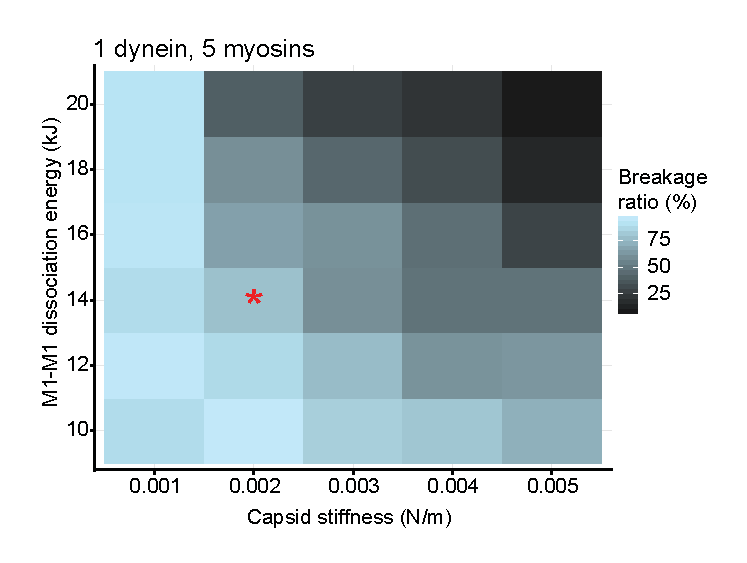
\includegraphics[width=0.8\textwidth, trim={0cm 0cm 0cm 0cm}, clip]{D_chapters/1_TugOfWar/SUPPLEMENTARYFIGURE1C.pdf}
\caption[Higher stiffness and dissociation energy of the capsid protein M1-M1 bond lead to a lower capsid breakage probability.]%
{Higher stiffness and dissociation energy of the capsid protein M1-M1 bond lead to a lower capsid breakage probability. \par
The red * symbol indicates stiffness and dissociation energy values reported in the literature, used for our simulations.}
\label{figure:StiffnessEnergy}
\end{center}
\end{figure}